\section{\textbf{Propuesta de Proyecto}}
\subsection{Planteamiento del Problema}
El c\'alculo de la similitud en series temporales ha sido un tema muy estudiado en la \'ultima d\'ecada \cite{rulediscovery}. La precisi\'on, la velocidad de c\'omputo y la tolerancia al ruido, son factores claves (particularmente en conjuntos de datos grandes y complejos) a la hora de elegir una medida de distancia robusta para comparar dos series de tiempo de largo n \cite{multidimensional}.\par
En la literatura, la medida de distancia m\'as utilizada para comparar series temporarles es sin duda la distancia \textit{Euclideana} (o alguna de sus variaciones). Dicha medida es muy utilizada en el descubrimiento y la comparaci\'on de reglas motif o patrones en series temporales \cite{motifs}\cite{patterns}.\par
Existen pruebas emp\'iricas fiables, que demuestran que la distancia Euclideana es muy competitiva e incluso superior a medidas mucho m\'as complejas en una amplia variedad de dominios, particularmente cuando el conjunto de datos se vuelve cada vez m\'as grande \cite{distancecomparison}\cite{timewarpingindexing}.\par
Sin embargo, algunos aportes m\'as recientes al estado del arte indican que  \textit{Dynamic Time Warping}, en una o varias dimensiones, puede incluso comportarse de forma m\'as robusta y estable que la distancia \textit{Euclideana} \cite{keogh}. Este argumento se soporta principalmente en la sensibilidad conocida que presenta la distancia \textit{Euclideana} ante la presencia de ruido, pero fundamentalmente y por su naturaleza lineal \cite{euclidean}, intolerante ante peque\~nas distorciones observadas al comparar dos series temporales desfasadas con respecto al eje tiempo \cite{DTWcubicsplineinterpolation}.\par
Por \'ultimo, la presencia de ruido y de valores faltantes en los datos de una serie de tiempo, son problemas dif\'iciles de tratar; lo que s\'i es seguro, es que son retos inevitables, pr\'acticamente inherentes, que al igual que las limitaciones de las medidas de distancia, deben abordarse previo al an\'alisis y que, finalmente definen el planteamiento del problema \cite{noise}.\par
El problema anteriormente planteado, se atacar\'a mediante la siguiente propuesta de investigaci\'on.
\subsection{Propuesta del Proyecto}
Apoyados en la premisa anterior, el proyecto pretende estudiar el nivel de acierto obtenido como resultado del descubrimiento de \textit{\enquote{reglas significativas}} en series de tiempo, utilizando \textit{Cubic Spline Interpolation} como una medida alternativia de distancia aparentemente superior a la distancia \textit{Euclideana}, principalmente ante la presen\-cia de distorciones en el conjunto de datos y otras limitaciones ya planteadas.\par
El proyecto se enfoca en remplazar la distancia Euclideana y probar que la utilizaci\'on de otras medidas de distancia (particularmente el uso de \textit{Cubic Spline Interpolation}) pueden ser mucho m\'as tolerantes al ruido y a\'un as\'i, garantizar al menos el mismo nivel de acierto en el descubrimiento de reglas significativas en series temporales.
\subsection{Trabajos Relacionados}
La presente propuesta de investigaci\'on se basa en trabajo de Mohammad Shokoohi-Yekta et al \cite{main}, quienes proponen una serie de nuevos algoritmos que permiten el des\-cubrimiento veloz de reglas significativas de alta calidad a partir de grandes conjuntos de datos, las cuales, pueden predecir la ocurrencia de eventos futuros.\par
Es importante destacar el hecho de que a pesar de que otras medidas de distancia fueron evaluadas (se menciona por ejemplo: DTW, Swale, Spade y ERP), \textit{\textbf{los algoritmos propuestos en \cite{main} utilizan la distancia Euclideana}} para la identificaci\'on de reglas motif y su selecci\'on posterior como reglas significativas.\par
A diferencia de otras propuestas mencionadas a continuaci\'on, el trabajo propuesto en \cite{main}, se basa en el descubrimiento de reglas motif con respecto a \textit{la forma}, para vaticinar los eventos futuros. En contraposici\'on, los trabajos anteriores intentan lograr predicciones basadas en los \textit{valores actuales} del flujo de datos \cite{others}.\par
En una secuencia de trabajos que culminaron en \cite{elasticrules}, Park y Chu, investigaron un mecanismo para hallar reglas sobre series de tiempo. Sin embargo, el algoritmo \'unicamente es valorado con respecto a la velocidad y datos aleatorios (\textit{random walk data}). No se presentaron pruebas de que el algoritmo pudiera en realidad encontrar las reglas generalizables en series de tiempo.\par
Los trabajos de Wu y colegas en \cite{eventdriven}, tambi\'en utilizan representaciones lineales de segmentos para apoyar el descubrimiento de reglas en series de tiempo. Ellos probaron su algoritmo sobre datos financieros reales, reportando aproximadamente un 68\% de \enquote{correcci\'on de la predicci\'on de la tendencia de datos} sobre la serie temporal. Curiosamente, sin embargo, los autores corrieron su algoritmo en datos proporcionados por otros y obtuvieron exactamente los mismos resultados.\\\\
\textbf{Acerca de los algoritmos propuestos en \cite{main}}\par
Una vez m\'as, es importante subrayar que en nuestra propuesta, se busca la modi\-ficaci\'on de dos algoritmos propuestos en \cite{main}, particularmente el reemplazo de la medida de distancia Euclideana. Ambos algoritmos ser\'an explicados a continuaci\'on en las tablas 1 y 2.\par
En la siguiente tabla, se explica el seudoc\'odigo del primer algoritmo llamado \enquote{\textit{\textbf{Find Antecedent Candidates}}}. Este algoritmo, sirve para la b\'usqueda de reglas motif (potenciales reglas significativas).\par 
Como se detalla en la tabla 1, el primer algoritmo 	recibe los siguientes argumentos: un segmento subsecuente $R$ extrac\'ido de la serie temporal $T$ y un punto de divisi\'on $sp$, que es simplemente un n\'umero entre cero y uno, utilizado para dividir los segmentos antecedentes y consecuentes de la regla \cite{main}.\par
El algoritmo devolver\'a las ubicaciones de los segmentos antecedentes encontrados en $T$, ordenados por las distancias a partir de los $R$ segmentos antecedentes almacenados y retornados como \textit{ac} \cite{main}.
\begin{center}
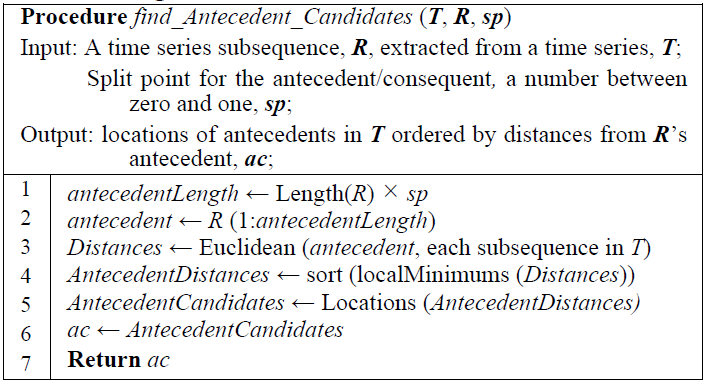
\includegraphics[scale=0.7]{antecedent.png}\\
\vspace*{10pt}
\footnotesize{\textbf{Tabla 1.} Seudoc\'odigo del algoritmo \enquote{Find Antecedent Candidates}.}
\end{center}
Como se observa en la linea 3 del algoritmo, la distancia Euclideana es implementada para el c\'omputo de las medidas de distancia, para encontrar \enquote{segmentos antecedentes} en cada subsecuencia de la serie temporal $T$ \cite{main}.\par
En la tabla 2, por su parte, se muestra el seudoc\'odigo del segundo algoritmo llamado \enquote{\textit{\textbf{Rule Bit Saves}}}.\par 
Este algoritmo, recibe como argumento, un segmento o subsecuencia $R$ extra\'ido de la serie temporal $T$, un punto de divisi\'on $sp$, que es un n\'umero entre cero y uno, el n\'umero de instancias de $R$ que ser\'an seleccionadas se almacenar\'an en $n$, la ubicaci\'on del segmento antecedente en la serie temporal $T$ ordenada por las distancias a partir de los segmentos antecedentes $R$ y finalmente el $maxlag$ o tiempo m\'aximo de rezago.\par El algoritmo devolver\'a como resultado el n\'umero total de bits ahorrados, es decir, la calificaci\'on acumulada de la regla motif (segmento $R$) con respecto a capacidad predictiva sobre la serie temporal $T$ \cite{main}.\par
\begin{center}
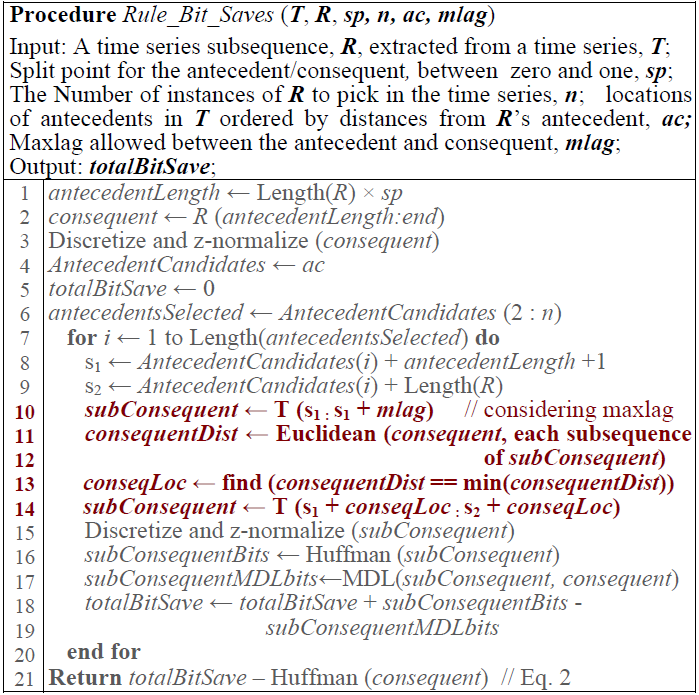
\includegraphics[scale=0.7]{rulebitsaves.png}\\
\vspace*{10pt}
\footnotesize{\textbf{Tabla 2.} Seudoc\'odigo del algoritmo \enquote{Rule Bit Save}.}
\end{center}
En la l\'inea 11 de la tabla 2, se observa claramente el uso de la distancia Euclideana para calcular la distancia entre entre el segmento consecuente, para cada occurrencia del segmento subsecuente $R$ que sea encontrado en $T$  \cite{main}.\par
Es importante resaltar el uso de MDL (Minimun Description Length, por sus siglas en Ingl\'es), en la l\'inea 17, inspirada en la estrategia de b\'usqueda m\'as simple posible, que eval\'ua las potenciales reglas significativas, con base en cuan bien pueden comprimir los datos \cite{main}.
\subsection{Hip\'otesis}
Con base en la definici\'on del problema y en la propuesta de proyecto, se define la siguiente hip\'otesis:\par
\textbf{\textit{El uso de la medida de distancia \textit{Cubic Spline Interpolation}, mejora el nivel de exactitud en los algoritmos \textit{\textbf{\enquote{Rule Bit Saves}}} y \textit{\textbf{\enquote{Find Antecedent Candidates}}} propuestos por Mohammad Shokoohi-Yekta y colaboradores, en el hallazgo de reglas significativas en series de tiempo complejas y en presencia de ruido.}} 
\subsection{M\'etricas}
El an\'alisis comparativo de los niveles de exactitud obtenidos a partir de la ejecuci\'on de los algoritmos seg\'un la distancia utilizada, requerir\'a de las siguientes m\'etricas:
\begin{itemize}
\item \textbf{Exactitud (Q):}
\begin{equation}
 \frac{Total\_Aciertos} {Total\_Predicciones}
\end{equation}
\end{itemize}
En el caso m\'as general, se utilizar\'a inicialmente la distancia Euclideana entre la parte consecuente predicha y las \textit{\textbf{F}} ubicaciones halladas desde donde la regla fue disparada, un valor denotado como \textit{\textbf{\enquote{Ferror}}}, tambi\'en conocido como la \textit{media cuadr\'atica}.\par
Sobre el mismo conjunto de prueba, y mediante el uso del mismo segmento consecuente de la regla, se disparar\'a aleatoriamente \textit{\textbf{F}} veces y se medir\'a la distancia \textit{Euclediana} (Cubic Spline Interpolation y otras ya mencionadas en el marco te\'orico), entre el segmento consecuente predicho y la ubicaciones aleatorias F.\par
Ese valor ser\'a denotado como \textit{\textbf{Rerror}} (el cual, se promediar\'a entre aproximadamente 1000 ejecuciones aleatorias).\par
En resumen, la medida de calidad reportada puede definirse como: 
\begin{equation} 
Q = \frac{Ferror}{Rerror} 
\end{equation}
Los valores cercanos a uno, sugieren que las reglas a prueba, no se consideran mejores que las encontradas en la estimaci\'on aleatoria. Los valores significativamente menores a uno, indican que la regla en efecto encuentra una estructura verdadera en los datos. En la mayor\'ia de los experimientos se utilizar\'a un retraso m\'aximo (\textit{\textbf{maxlag}}) \cite{main} igual a cero.
\subsection{Justificaci\'on del Proyecto}
La realizaci\'on de este proyecto es importante, porque a trav\'es de sus resultados se podr\'ian llegar a obtener los siguientes beneficios:
\begin{itemize}
\item {\textbf{\textbf{Un aporte al estado del arte}}. El estudio del estado del arte realizado indica que \enquote{Cubic Spline Interpolation}, como medida de distancia, no ha sido utilizado a\'un en algoritmos para el descubrimiento de reglas significativas sobre series temporales. La idea es, por ende, prometedora e innovadora y podr\'ia tener un impacto significativo sobre el rendimiento de algoritmos existentes que actualmente utilizan otras medidas de distancia m\'as utilizadas como por ejemplo, la distancia \textit{Eucledeana}.}
\item {\textbf{Ataca un problema de investigaci\'on real}. Muchas de las aplicaciones producto del an\'alisis de series temporales, son posibles a partir del descubrimiento de reglas \textit{motif} y su uso posterior sobre el conjunto de datos \cite{main}. El descubrimiento de dichos patrones en series temporales, se puede resumir a un problema de \textit{similitud}. El c\'omputo de la similitud (o disimilitud) se obtiene a partir de la medida de distancia entre los puntos de datos de las series temporales \cite{main}. Mientras m\'as eficiente y robusta sea la medida de distancia, mejor ser\'a el c\'alculo de la similitud y por ende, mejores reglas \textit{motif} se obtendr\'an. Como consecuencia de lo anterior, la precisi\'on, la velocidad del c\'omputo y la tolerancia al ruido ser\'an superior y por consiguiente, la calidad predictiva de la regla sobre el conjunto de datos ser\'a mucho m\'as fiable \cite{measurements}.}
\item {\textbf{Las potenciales aplicaciones y su impacto en la sociedad}. Como se desarroll\'o en el marco te\'orico, las aplicaciones de la miner\'ia sobre series temporales son amplias y diversas  \cite{main}. Las predicciones de corto plazo mediante el uso de reglas significativas en campos triviales como el an\'alisis del mercado de accio\-nes, el estudio de las condiciones meteorol\'ogicas (por ejemplo, el incremento del tiempo promedio de alerta de tornados \cite{weatherforcasting}) son cada d\'ia m\'as utilizadas. En rob\'otica, por ejemplo, se han realizado avances significativos en la exploraci\'on de la anticipaci\'on (predicciones de corto plazo) de las fuerzas futuras percibidas por un robot con base en las intenciones motoras de otro agente y as\'i adaptar su movimiento, ejecutando un nuevo plan de acci\'on \cite{robotics}.}
\end{itemize}